\section{Inequação do 2° grau}

\begin{definition}
Uma \textdef{inequação do segundo grau} é uma relação de uma das formas
a seguir:
%
\begin{gather*}
ax^2 +bx + c <0;\\
ax^2 +bx + c>0;\\
ax^2 +bx + c \le 0;\\
ax^2 +bx + c \ge 0;\\
\end{gather*}
%
onde $a, b, c \in \R$, com $ a \ne 0$.
\end{definition}

\begin{example}
Resolva as seguintes inequações: $x^2 -3x +2 > 0$; $x^2 -3x +2 \le 0$.
\end{example}

\begin{solution}
Observe que: 
%
\begin{align*}
x^2-3x+2=\prn{x-2}\prn{x-1}>0
\end{align*}
%
\noindent logo, teremos:

\begin{figure}[H]
\centering
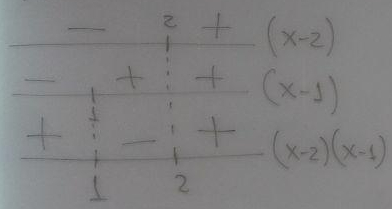
\includegraphics{\imgdirfromsection/[ok]photo_2018-08-24_22-55-35.jpg}
\caption{}
\end{figure}

Assim, $S = \set{x \in \R \tq{x<1 \text{ ou } x>2}}$. Ademais, a solução $\bar{S}$ para a inequação $x^2-3x+2\le0$ será:
%
\begin{align*}
\bar{S} &= \set{x \in \R \tq x \ge 1 \text{ e } x \le 2} \\
		&= \set{x \in \R \tq 1 \le x \le 2} 
\end{align*}
\end{solution}

\begin{example}
Prove que a soma de um número positivo com seu inverso é sempre maior ou igual a 2.
\end{example}

\begin{proof}
Queremos provar que $x+1/x\ge 2$, para todo $x > 0$. Note que:
%
\begin{align*}
x+\dfrac{1}{x}\ge 2 &\iff \dfrac{x^2+1-2x}{x} \\
		&\iff \dfrac{\prn{x-1}^2}{x}
\end{align*}

\begin{figure}[H]
\centering
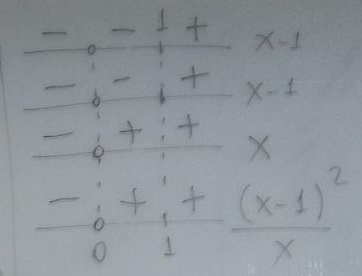
\includegraphics{\imgdirfromsection/[ok]photo_2018-08-24_22-55-35(2).jpg}
\caption{}
\end{figure}

Logo, para que $x+1/x\ge 2$, é necessário e suficiente que $x > 0$, ou seja, $x$ é positivo.
\end{proof}